\documentclass[tikz,border=5pt]{standalone}
\usepackage[utf8]{inputenc}
\usepackage[T1]{fontenc}
\usepackage{amsmath,amssymb}
\usepackage{lmodern}
\usetikzlibrary{arrows.meta}

\definecolor{boxbg}{HTML}{1d1d1f}
\definecolor{amberbg}{HTML}{2c2214}
\definecolor{lighttext}{HTML}{f5f5f7}
\definecolor{subtext}{HTML}{d1d1d6}
\definecolor{muted}{HTML}{86868b}
\definecolor{gridline}{HTML}{48484a}
\definecolor{amber}{HTML}{ff9f0a}
\definecolor{amberlight}{HTML}{ffd60a}
\definecolor{redaccent}{HTML}{ff453a}
\definecolor{redlight}{HTML}{ff6961}

\begin{document}
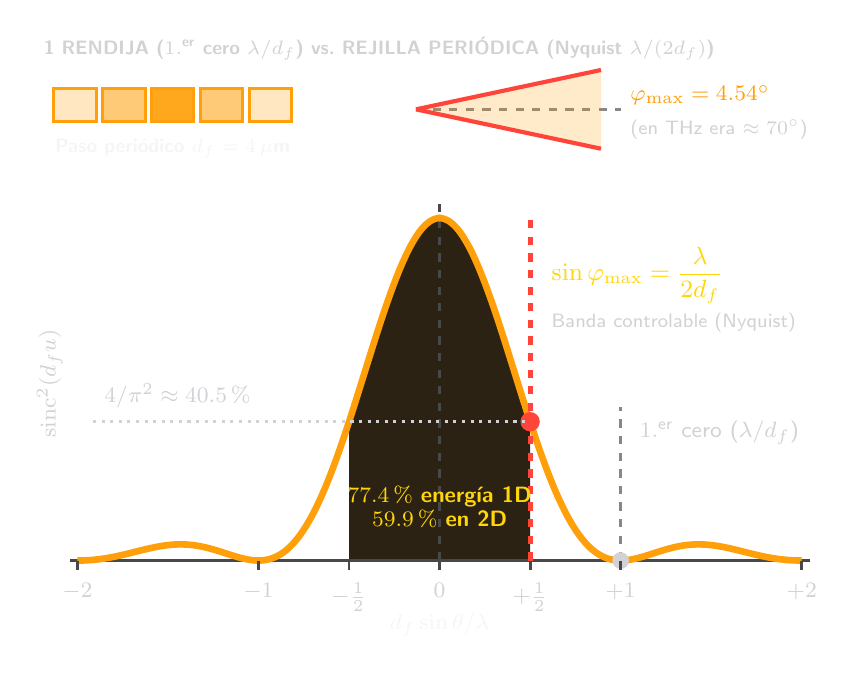
\begin{tikzpicture}[font=\sffamily,>=Stealth]

% ===================== TIRA SUPERIOR: REJILLA vs CONO =====================
\node[anchor=west,text=subtext,font=\sffamily\scriptsize\bfseries] at (0,7.55)
  {1 RENDIJA ($1.^{\text{er}}$ cero $\lambda/d_f$) vs.\ REJILLA PERIÓDICA (Nyquist $\lambda/(2d_f)$)};

% 5 píxeles periódicos
\foreach \i/\op in {0/0.25, 1/0.55, 2/0.92, 3/0.55, 4/0.25} {
  \fill[amber,opacity=\op] ({0.25 + 0.62*\i}, 6.62) rectangle ({0.25 + 0.62*\i + 0.54}, 7.05);
  \draw[amber,line width=1.1pt] ({0.25 + 0.62*\i}, 6.62) rectangle ({0.25 + 0.62*\i + 0.54}, 7.05);
}
\node[text=lighttext,font=\sffamily\scriptsize\bfseries] at (1.76,6.28) {Paso periódico $d_f = 4\,\mu\text{m}$};

% Cono estrecho 4.54 grados
\draw[muted,dashed,line width=0.9pt] (4.85,6.78) -- (7.45,6.78);
\fill[amber,opacity=0.22] (4.85,6.78) -- (7.20,7.28) -- (7.20,6.28) -- cycle;
\draw[redaccent,line width=1.5pt] (4.85,6.78) -- (7.20,7.28);
\draw[redaccent,line width=1.5pt] (4.85,6.78) -- (7.20,6.28);
\node[anchor=west,text=amber,font=\sffamily\footnotesize\bfseries] at (7.45,6.96)
  {$\varphi_{\max} = 4.54^\circ$};
\node[anchor=west,text=subtext,font=\sffamily\scriptsize] at (7.45,6.52)
  {(en THz era $\approx 70^\circ$)};

% ===================== GRÁFICA EXACTA SINC^2 =====================
% Origen (5.15, 1.05): x in [-2, 2] -> escala 1 u = 2.30 cm (ancho total 9.2 cm: 0.55 .. 9.75)
% y in [0, 1] -> escala 1 u = 4.35 cm (alto total 4.35 cm: 1.05 .. 5.40)
\begin{scope}[shift={(5.15,1.05)}]
  % Área sombreada Nyquist [-0.5, +0.5]
  \fill[amberbg]
    (-1.15,0) --
    plot[domain=-0.5:-0.002,samples=40] ({2.30*\x}, {4.35*pow(sin(deg(pi*\x))/(pi*\x),2)}) --
    (0,4.35) --
    plot[domain=0.002:0.5,samples=40] ({2.30*\x}, {4.35*pow(sin(deg(pi*\x))/(pi*\x),2)}) --
    (1.15,0) -- cycle;

  % Eje horizontal y vertical central
  \draw[gridline,line width=1.2pt] (-4.70,0) -- (4.70,0);
  \draw[gridline,dashed,line width=0.9pt] (0,0) -- (0,4.55);

  % Curva sinc^2(x) EXACTA en dos mitades unidas en (0,1)
  \draw[amber,line width=2.4pt]
    plot[domain=-2.0:-0.002,samples=110] ({2.30*\x}, {4.35*pow(sin(deg(pi*\x))/(pi*\x),2)}) --
    (0,4.35) --
    plot[domain=0.002:2.0,samples=110] ({2.30*\x}, {4.35*pow(sin(deg(pi*\x))/(pi*\x),2)});

  % Línea roja Nyquist en x = +0.5 -> sinc^2(0.5) = 4/pi^2 = 0.40528
  \draw[redaccent,dashed,line width=1.8pt] (1.15,0) -- (1.15,4.35);
  \fill[redaccent] (1.15,{4.35*0.40528}) circle (3.5pt);

  % Línea horizontal 4/pi^2 = 40.5 %
  \draw[subtext,dotted,line width=1.1pt] (-4.40,{4.35*0.40528}) -- (1.15,{4.35*0.40528});
  \node[anchor=south west,text=subtext,font=\sffamily\footnotesize\bfseries] at (-4.38,{4.35*0.40528 + 0.05})
    {$4/\pi^2 \approx 40.5\,\%$};

  % Línea gris primer cero en x = +1.0
  \draw[muted,dashed,line width=1.2pt] (2.30,0) -- (2.30,1.95);
  \fill[subtext] (2.30,0) circle (3pt);

  % Etiquetas dentro de la gráfica
  \node[anchor=west,text=amberlight,font=\sffamily\small\bfseries] at (1.30,3.62)
    {$\sin\varphi_{\max} = \dfrac{\lambda}{2d_f}$};
  \node[anchor=west,text=subtext,font=\sffamily\scriptsize] at (1.30,3.02)
    {Banda controlable (Nyquist)};

  \node[anchor=west,text=subtext,font=\sffamily\footnotesize] at (2.42,1.62)
    {$1.^{\text{er}}$ cero ($\lambda/d_f$)};

  \node[text=amberlight,font=\sffamily\footnotesize\bfseries,align=center] at (0,0.68)
    {$77.4\,\%$ energía 1D\\[-1pt]$59.9\,\%$ en 2D};

  % Ticks en x
  \foreach \val/\lbl in {-2/$-2$, -1/$-1$, -0.5/$-\tfrac{1}{2}$, 0/$0$, 0.5/$+\tfrac{1}{2}$, 1/$+1$, 2/$+2$} {
    \draw[gridline,line width=1pt] ({2.30*\val},0) -- ({2.30*\val},-0.12);
    \node[anchor=north,text=subtext,font=\sffamily\footnotesize] at ({2.30*\val},-0.16) {\lbl};
  }

  % Etiquetas de ejes
  \node[text=lighttext,font=\sffamily\footnotesize\bfseries] at (0,-0.82)
    {$d_f \sin\theta / \lambda$};
  \node[rotate=90,text=subtext,font=\sffamily\footnotesize\bfseries] at (-4.95,2.25)
    {$\operatorname{sinc}^2(d_f u)$};
\end{scope}

\end{tikzpicture}
\end{document}
